\appendix
%\renewcommand\thesection{\Alph{section}}
\addcontentsline{toc}{chapter}{Anhang}
\addtocontents{toc}{%
  %\protect\addtokomafont{chapterentry}{Anhang\ }
}
%\chapter{}
\refstepcounter{chapter}
\addcontentsline{toc}{section}{A\quad Referenzbilder}
\chaptermark{Referenzbilder}
\label{app:reference}
\section*{A\quad Referenzbilder}


\renewcommand{\mywidth}{0.17}
\begin{figure}[h!]
\subfloat[Referenz 1]{
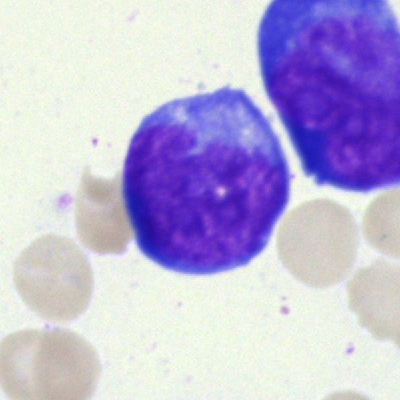
\includegraphics[width = \mywidth\textwidth]{pics/Anhang/single01}}
\quad
\subfloat[Referenz 2]{
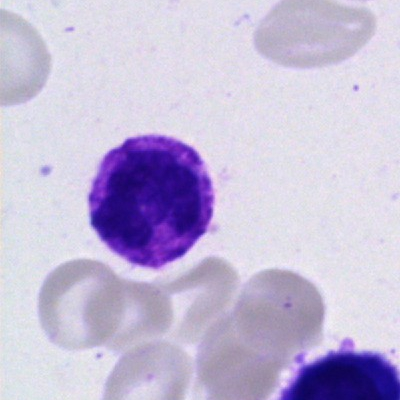
\includegraphics[width = \mywidth\textwidth]{pics/Anhang/single02}}
\quad
\subfloat[Referenz 3]{
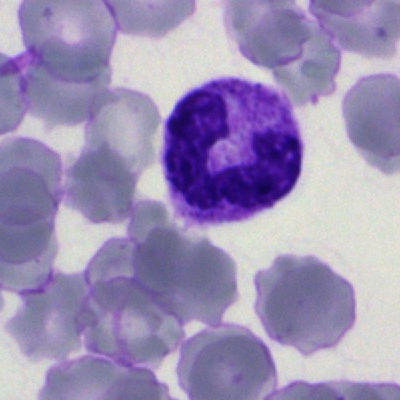
\includegraphics[width = \mywidth\textwidth]{pics/Anhang/single03}}
\quad
\subfloat[Referenz 4]{
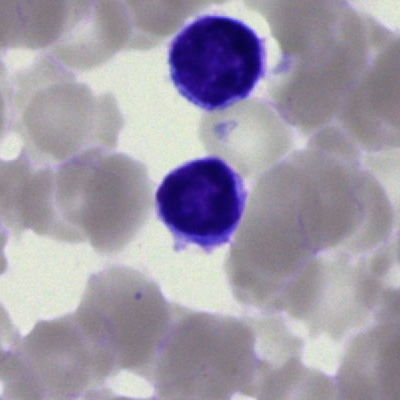
\includegraphics[width = \mywidth\textwidth]{pics/Anhang/single04}}
\quad
\subfloat[Referenz 5]{
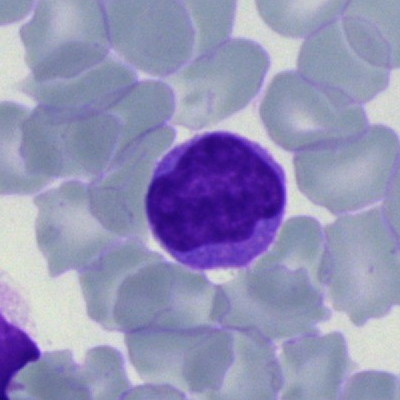
\includegraphics[width = \mywidth\textwidth]{pics/Anhang/single05}}
\quad
\subfloat[Referenz 6]{
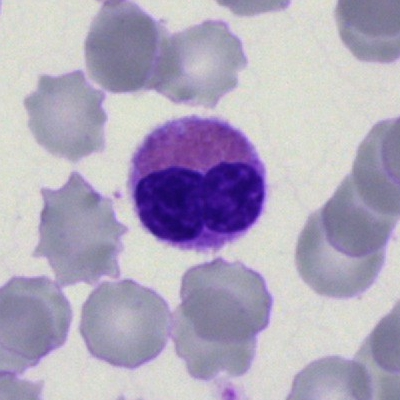
\includegraphics[width = \mywidth\textwidth]{pics/Anhang/single06}}
\quad
\subfloat[Referenz 7]{
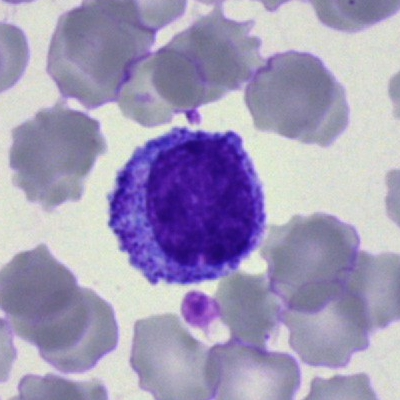
\includegraphics[width = \mywidth\textwidth]{pics/Anhang/single07}}
\quad
\subfloat[Referenz 8]{
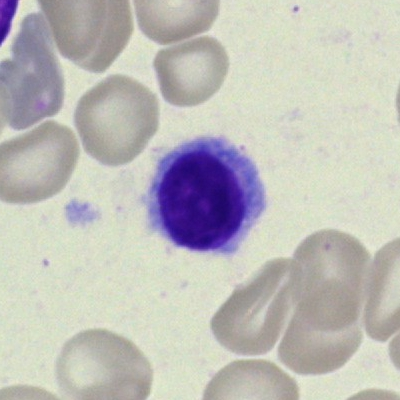
\includegraphics[width = \mywidth\textwidth]{pics/Anhang/single08}}
\quad
\subfloat[Referenz 9]{
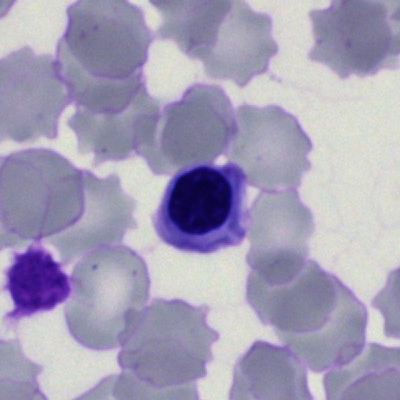
\includegraphics[width = \mywidth\textwidth]{pics/Anhang/single09}}
\quad
\subfloat[Referenz 10]{
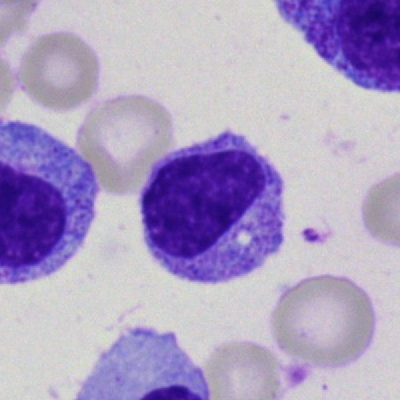
\includegraphics[width = \mywidth\textwidth]{pics/Anhang/single10}}
\quad
\subfloat[Referenz 11]{
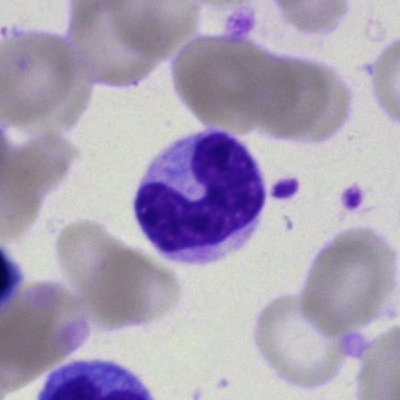
\includegraphics[width = \mywidth\textwidth]{pics/Anhang/single11}}
\quad
\subfloat[Referenz 12]{
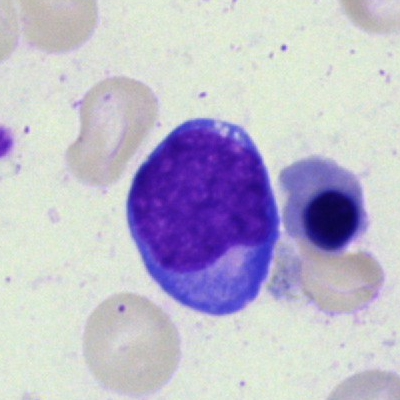
\includegraphics[width = \mywidth\textwidth]{pics/Anhang/single12}}
\quad
\subfloat[Referenz 13]{
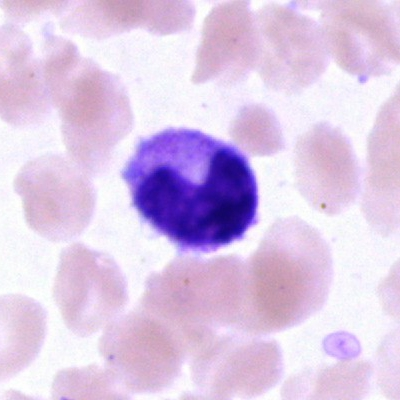
\includegraphics[width = \mywidth\textwidth]{pics/Anhang/single13}}
\quad
\subfloat[Referenz 14]{
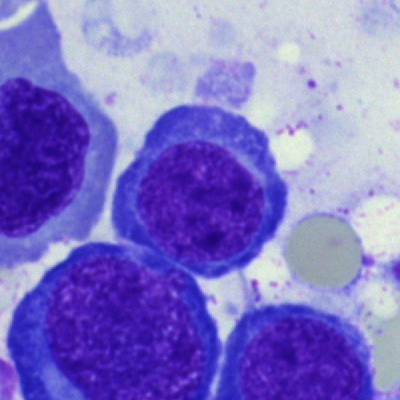
\includegraphics[width = \mywidth\textwidth]{pics/Anhang/single14}}
\quad
\subfloat[Referenz 15]{
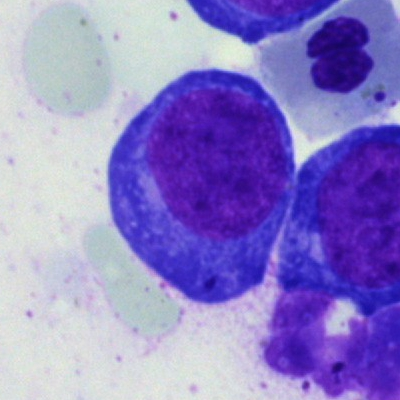
\includegraphics[width = \mywidth\textwidth]{pics/Anhang/single15}}
\caption{Alle Referenzbilder\label{fig:all_references}}
\end{figure}

\begin{table}[h!]
\center
\caption{Zusammensetzung Referenzsets}
\begin{tabular}{|c|r|}
\hline
\textbf{Set} & \textbf{Zusammensetzung} \\ 
\hline
3 & 1-15 \\ 
\hline 
4 & ohne 1,10,11,14\\ 
\hline 
5 & 2,5,6,8,9,15 \\ 
\hline 
6 & 2,8,9 \\ 
\hline
7 & 1,2,4,10,12,14,15\\
\hline
\end{tabular} 
\end{table}

\clearpage
\addcontentsline{toc}{section}{B\quad �bersicht Wirkung Normalisierungsmethoden}
\refstepcounter{chapter}
\chaptermark{�bersicht Wirkung Normalisierungmethoden}
\label{app:norm}
\section*{B\quad �bersicht Wirkung Normalisierungmethoden}
\renewcommand{\mywidth}{0.17}
\begin{figure}[h!]
\center
\subfloat{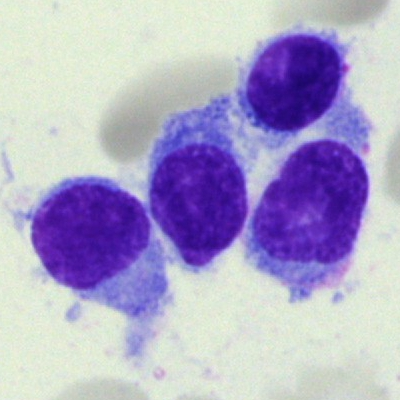
\includegraphics[width = \mywidth\textwidth]{pics/Anhang/B/01_or}}
\quad
\subfloat{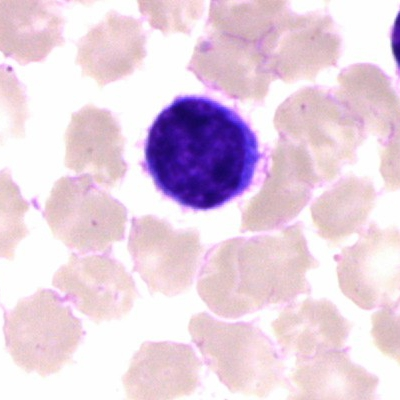
\includegraphics[width = \mywidth\textwidth]{pics/Anhang/B/02_or}}
\quad
\subfloat{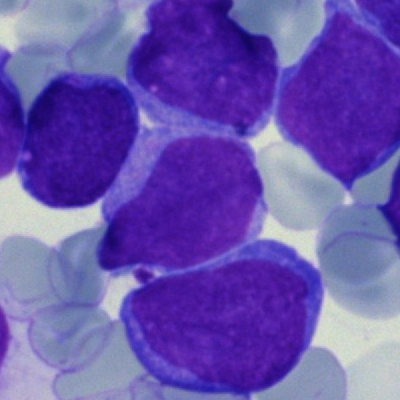
\includegraphics[width = \mywidth\textwidth]{pics/Anhang/B/03_or}}
\quad
\subfloat{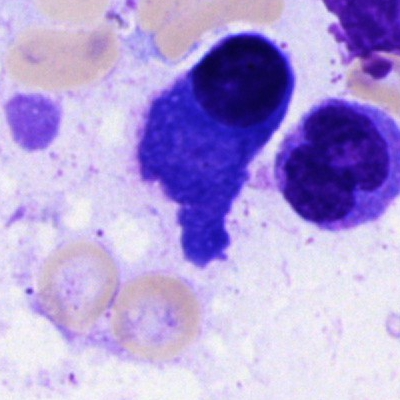
\includegraphics[width = \mywidth\textwidth]{pics/Anhang/B/04_or}}
\quad
\subfloat{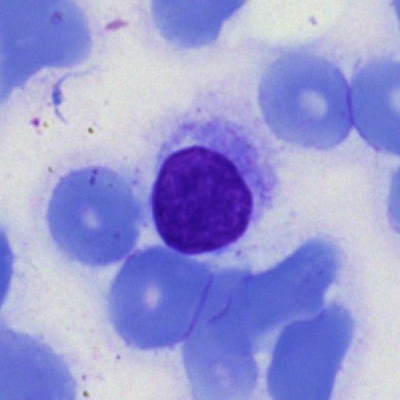
\includegraphics[width = \mywidth\textwidth]{pics/Anhang/B/05_or}}
\quad
\subfloat{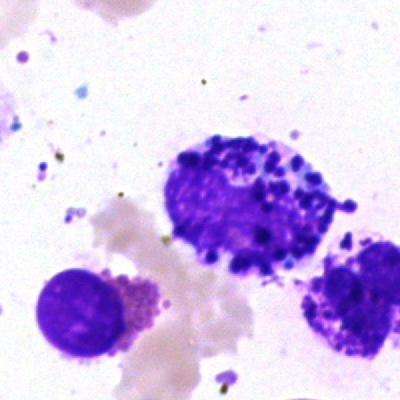
\includegraphics[width = \mywidth\textwidth]{pics/Anhang/B/06_or}}
\quad
\subfloat{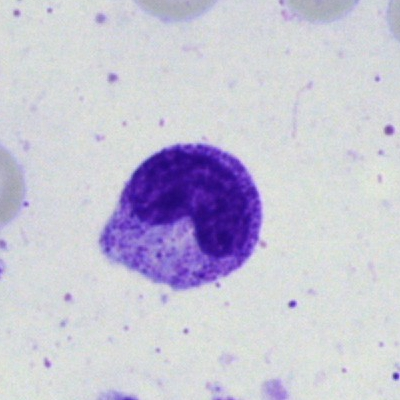
\includegraphics[width = \mywidth\textwidth]{pics/Anhang/B/07_or}}
\quad
\subfloat{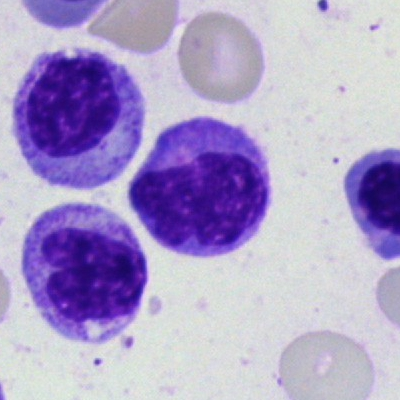
\includegraphics[width = \mywidth\textwidth]{pics/Anhang/B/08_or}}
\quad
\subfloat{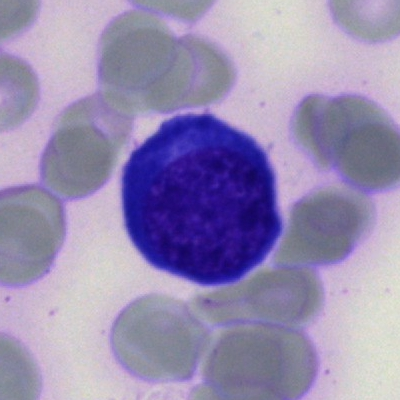
\includegraphics[width = \mywidth\textwidth]{pics/Anhang/B/09_or}}
\quad
\subfloat{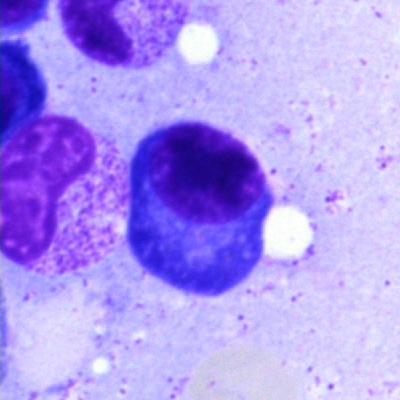
\includegraphics[width = \mywidth\textwidth]{pics/Anhang/B/10_or}}
\quad
\subfloat{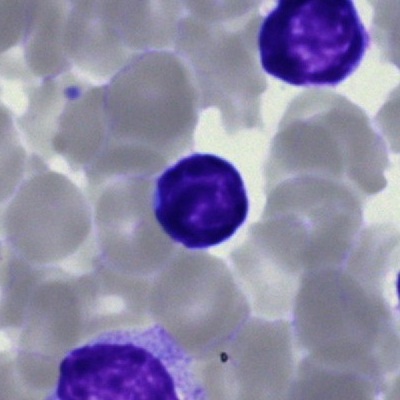
\includegraphics[width = \mywidth\textwidth]{pics/Anhang/B/11_or}}
\quad
\subfloat{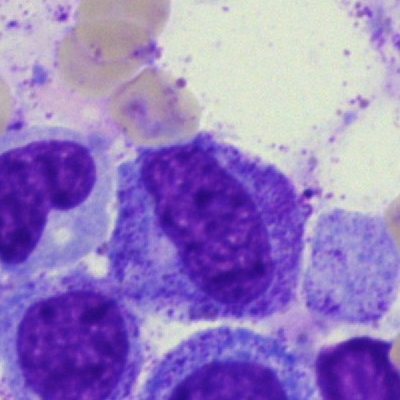
\includegraphics[width = \mywidth\textwidth]{pics/Anhang/B/12_or}}
\quad
\subfloat{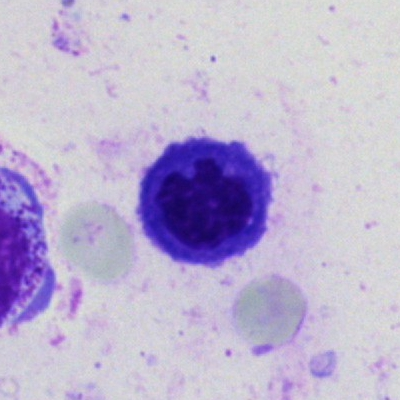
\includegraphics[width = \mywidth\textwidth]{pics/Anhang/B/13_or}}
\quad
\subfloat{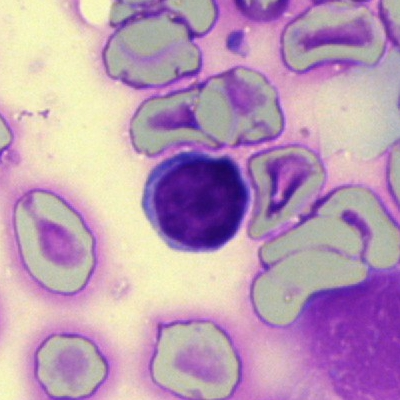
\includegraphics[width = \mywidth\textwidth]{pics/Anhang/B/14_or}}
\quad
\subfloat{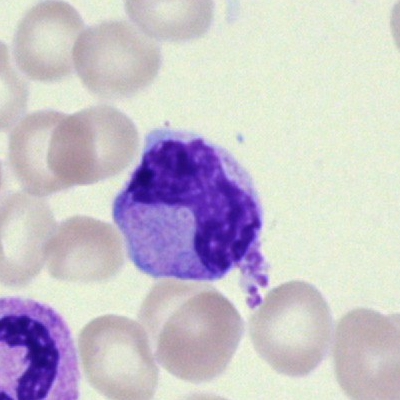
\includegraphics[width = \mywidth\textwidth]{pics/Anhang/B/15_or}}
\quad
\subfloat{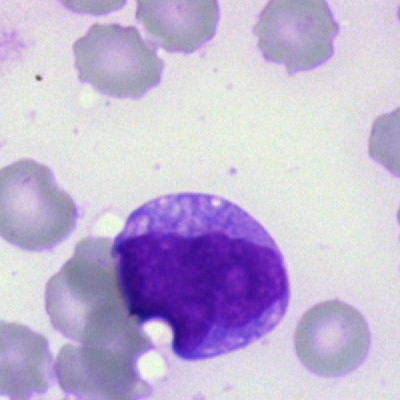
\includegraphics[width = \mywidth\textwidth]{pics/Anhang/B/16_or}}
\quad
\subfloat{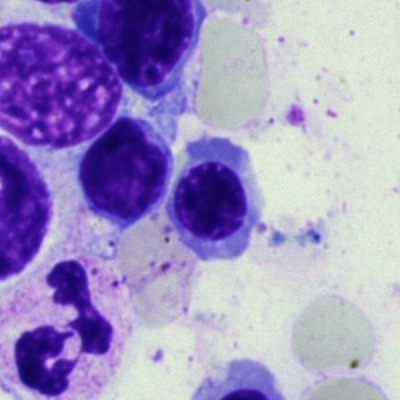
\includegraphics[width = \mywidth\textwidth]{pics/Anhang/B/17_or}}
\quad
\subfloat{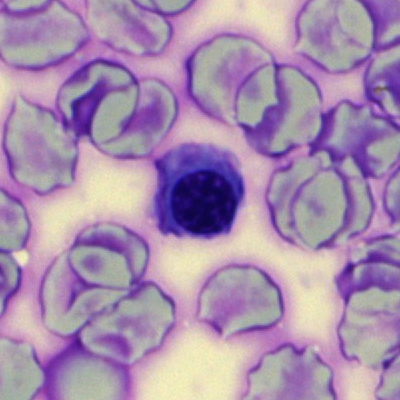
\includegraphics[width = \mywidth\textwidth]{pics/Anhang/B/18_or}}
\quad
\subfloat{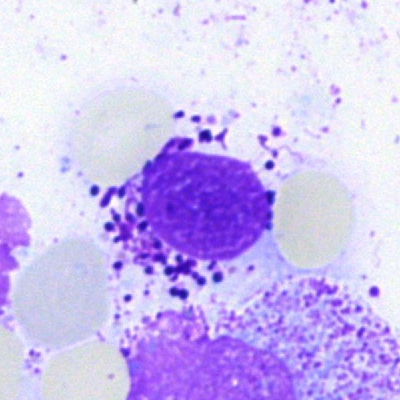
\includegraphics[width = \mywidth\textwidth]{pics/Anhang/B/19_or}}
\quad
\subfloat{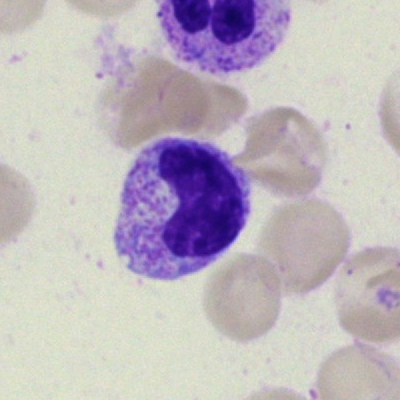
\includegraphics[width = \mywidth\textwidth]{pics/Anhang/B/20_or}}
\quad
\subfloat{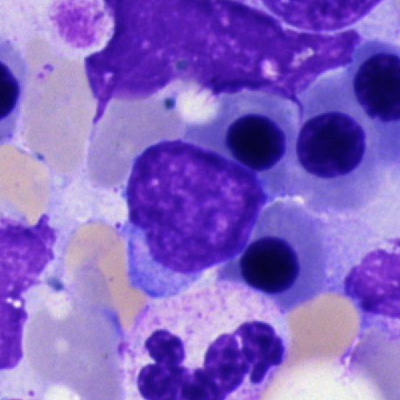
\includegraphics[width = \mywidth\textwidth]{pics/Anhang/B/21_or}}
\quad
\subfloat{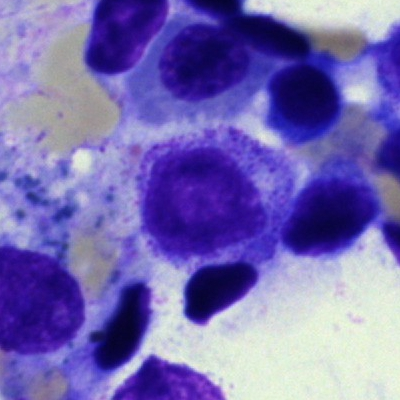
\includegraphics[width = \mywidth\textwidth]{pics/Anhang/B/22_or}}
\quad
\subfloat{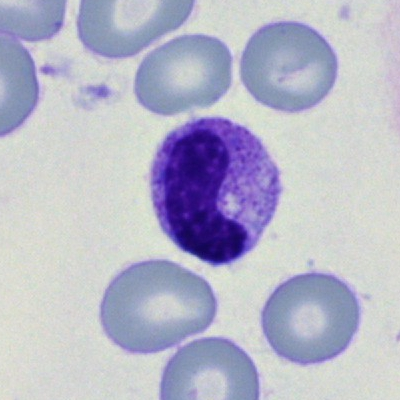
\includegraphics[width = \mywidth\textwidth]{pics/Anhang/B/23_or}}
\quad
\subfloat{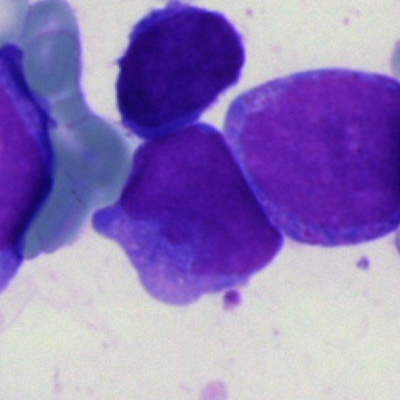
\includegraphics[width = \mywidth\textwidth]{pics/Anhang/B/24_or}}
\quad
\subfloat{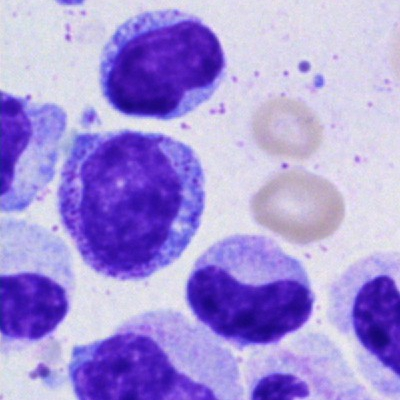
\includegraphics[width = \mywidth\textwidth]{pics/Anhang/B/25_or}}
\caption{Originalbilder\label{fig:25_original}}

\end{figure}

\begin{figure}[h!]
\center
\subfloat{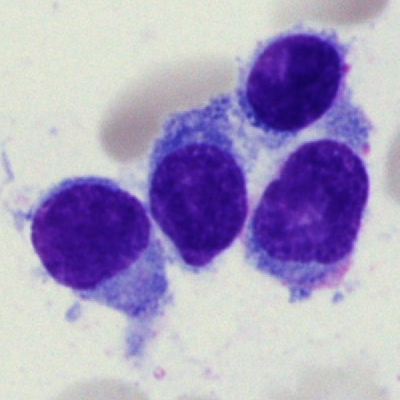
\includegraphics[width = \mywidth\textwidth]{pics/Anhang/B/01_gie}}
\quad
\subfloat{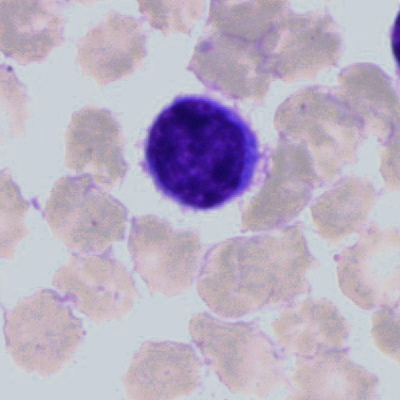
\includegraphics[width = \mywidth\textwidth]{pics/Anhang/B/02_gie}}
\quad
\subfloat{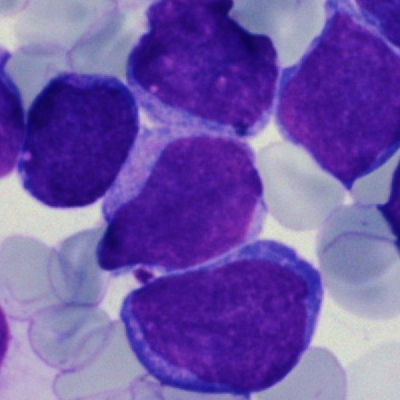
\includegraphics[width = \mywidth\textwidth]{pics/Anhang/B/03_gie}}
\quad
\subfloat{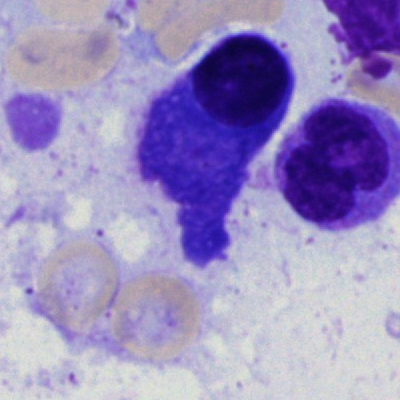
\includegraphics[width = \mywidth\textwidth]{pics/Anhang/B/04_gie}}
\quad
\subfloat{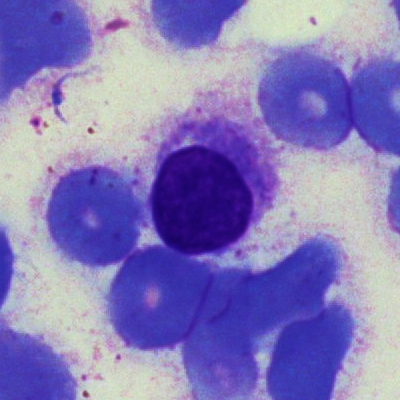
\includegraphics[width = \mywidth\textwidth]{pics/Anhang/B/05_gie}}
\quad
\subfloat{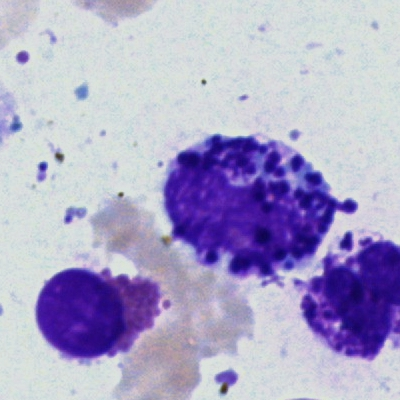
\includegraphics[width = \mywidth\textwidth]{pics/Anhang/B/06_gie}}
\quad
\subfloat{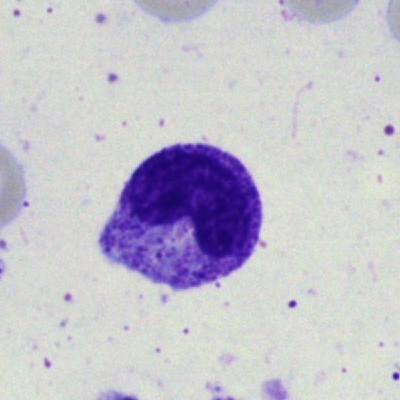
\includegraphics[width = \mywidth\textwidth]{pics/Anhang/B/07_gie}}
\quad
\subfloat{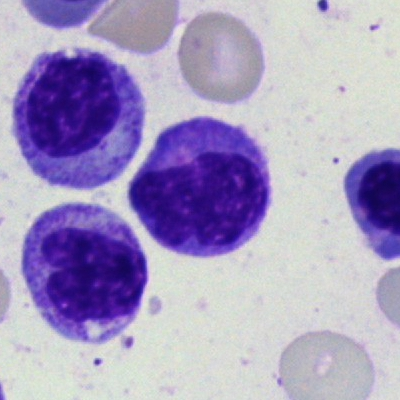
\includegraphics[width = \mywidth\textwidth]{pics/Anhang/B/08_gie}}
\quad
\subfloat{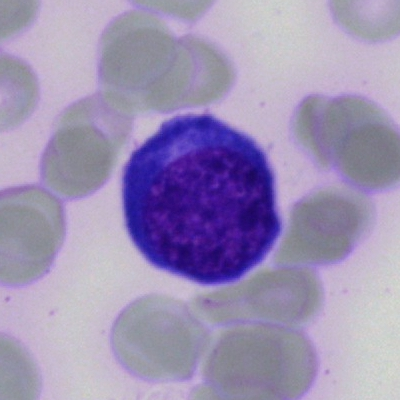
\includegraphics[width = \mywidth\textwidth]{pics/Anhang/B/09_gie}}
\quad
\subfloat{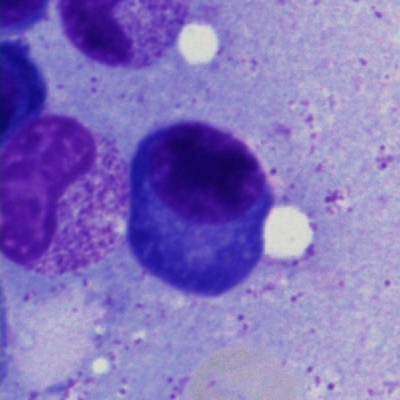
\includegraphics[width = \mywidth\textwidth]{pics/Anhang/B/10_gie}}
\quad
\subfloat{\includegraphics[width = \mywidth\textwidth]{pics/Anhang/B/11_gie}}
\quad
\subfloat{\includegraphics[width = \mywidth\textwidth]{pics/Anhang/B/12_gie}}
\quad
\subfloat{\includegraphics[width = \mywidth\textwidth]{pics/Anhang/B/13_gie}}
\quad
\subfloat{\includegraphics[width = \mywidth\textwidth]{pics/Anhang/B/14_gie}}
\quad
\subfloat{\includegraphics[width = \mywidth\textwidth]{pics/Anhang/B/15_gie}}
\quad
\subfloat{\includegraphics[width = \mywidth\textwidth]{pics/Anhang/B/16_gie}}
\quad
\subfloat{\includegraphics[width = \mywidth\textwidth]{pics/Anhang/B/17_gie}}
\quad
\subfloat{\includegraphics[width = \mywidth\textwidth]{pics/Anhang/B/18_gie}}
\quad
\subfloat{\includegraphics[width = \mywidth\textwidth]{pics/Anhang/B/19_gie}}
\quad
\subfloat{\includegraphics[width = \mywidth\textwidth]{pics/Anhang/B/20_gie}}
\quad
\subfloat{\includegraphics[width = \mywidth\textwidth]{pics/Anhang/B/21_gie}}
\quad
\subfloat{\includegraphics[width = \mywidth\textwidth]{pics/Anhang/B/22_gie}}
\quad
\subfloat{\includegraphics[width = \mywidth\textwidth]{pics/Anhang/B/23_gie}}
\quad
\subfloat{\includegraphics[width = \mywidth\textwidth]{pics/Anhang/B/24_gie}}
\quad
\subfloat{\includegraphics[width = \mywidth\textwidth]{pics/Anhang/B/25_gie}}
\caption[B-Spline nach Color Deconvolution mit Stainvektoren der Giemsa-F�rbung]{B-Spline nach Color Deconvolution mit Stainvektoren der Giemsa-F�rbung, Referenzset 5 (siehe Anhang \ref{app:reference})\label{fig:25_gie}}

\end{figure}

\begin{figure}[h!]
\center
\subfloat{\includegraphics[width = \mywidth\textwidth]{pics/Anhang/B/01_mac}}
\quad
\subfloat{\includegraphics[width = \mywidth\textwidth]{pics/Anhang/B/02_mac}}
\quad
\subfloat{\includegraphics[width = \mywidth\textwidth]{pics/Anhang/B/03_mac}}
\quad
\subfloat{\includegraphics[width = \mywidth\textwidth]{pics/Anhang/B/04_mac}}
\quad
\subfloat{\includegraphics[width = \mywidth\textwidth]{pics/Anhang/B/05_mac}}
\quad
\subfloat{\includegraphics[width = \mywidth\textwidth]{pics/Anhang/B/06_mac}}
\quad
\subfloat{\includegraphics[width = \mywidth\textwidth]{pics/Anhang/B/07_mac}}
\quad
\subfloat{\includegraphics[width = \mywidth\textwidth]{pics/Anhang/B/08_mac}}
\quad
\subfloat{\includegraphics[width = \mywidth\textwidth]{pics/Anhang/B/09_mac}}
\quad
\subfloat{\includegraphics[width = \mywidth\textwidth]{pics/Anhang/B/10_mac}}
\quad
\subfloat{\includegraphics[width = \mywidth\textwidth]{pics/Anhang/B/11_mac}}
\quad
\subfloat{\includegraphics[width = \mywidth\textwidth]{pics/Anhang/B/12_mac}}
\quad
\subfloat{\includegraphics[width = \mywidth\textwidth]{pics/Anhang/B/13_mac}}
\quad
\subfloat{\includegraphics[width = \mywidth\textwidth]{pics/Anhang/B/14_mac}}
\quad
\subfloat{\includegraphics[width = \mywidth\textwidth]{pics/Anhang/B/15_mac}}
\quad
\subfloat{\includegraphics[width = \mywidth\textwidth]{pics/Anhang/B/16_mac}}
\quad
\subfloat{\includegraphics[width = \mywidth\textwidth]{pics/Anhang/B/17_mac}}
\quad
\subfloat{\includegraphics[width = \mywidth\textwidth]{pics/Anhang/B/18_mac}}
\quad
\subfloat{\includegraphics[width = \mywidth\textwidth]{pics/Anhang/B/19_mac}}
\quad
\subfloat{\includegraphics[width = \mywidth\textwidth]{pics/Anhang/B/20_mac}}
\quad
\subfloat{\includegraphics[width = \mywidth\textwidth]{pics/Anhang/B/21_mac}}
\quad
\subfloat{\includegraphics[width = \mywidth\textwidth]{pics/Anhang/B/22_mac}}
\quad
\subfloat{\includegraphics[width = \mywidth\textwidth]{pics/Anhang/B/23_mac}}
\quad
\subfloat{\includegraphics[width = \mywidth\textwidth]{pics/Anhang/B/24_mac}}
\quad
\subfloat{\includegraphics[width = \mywidth\textwidth]{pics/Anhang/B/25_mac}}
\caption[B-Spline nach Color Deconvolution mit Stainvektoren nach Macenko]{B-Spline nach Color Deconvolution mit Stainvektoren nach Macenko, Referenzset 5 (siehe Anhang \ref{app:reference})\label{fig:25_mac}}

\end{figure}

\begin{figure}[h!]
\center
\subfloat{\includegraphics[width = \mywidth\textwidth]{pics/Anhang/B/01_fix}}
\quad
\subfloat{\includegraphics[width = \mywidth\textwidth]{pics/Anhang/B/02_fix}}
\quad
\subfloat{\includegraphics[width = \mywidth\textwidth]{pics/Anhang/B/03_fix}}
\quad
\subfloat{\includegraphics[width = \mywidth\textwidth]{pics/Anhang/B/04_fix}}
\quad
\subfloat{\includegraphics[width = \mywidth\textwidth]{pics/Anhang/B/05_fix}}
\quad
\subfloat{\includegraphics[width = \mywidth\textwidth]{pics/Anhang/B/06_fix}}
\quad
\subfloat{\includegraphics[width = \mywidth\textwidth]{pics/Anhang/B/07_fix}}
\quad
\subfloat{\includegraphics[width = \mywidth\textwidth]{pics/Anhang/B/08_fix}}
\quad
\subfloat{\includegraphics[width = \mywidth\textwidth]{pics/Anhang/B/09_fix}}
\quad
\subfloat{\includegraphics[width = \mywidth\textwidth]{pics/Anhang/B/10_fix}}
\quad
\subfloat{\includegraphics[width = \mywidth\textwidth]{pics/Anhang/B/11_fix}}
\quad
\subfloat{\includegraphics[width = \mywidth\textwidth]{pics/Anhang/B/12_fix}}
\quad
\subfloat{\includegraphics[width = \mywidth\textwidth]{pics/Anhang/B/13_fix}}
\quad
\subfloat{\includegraphics[width = \mywidth\textwidth]{pics/Anhang/B/14_fix}}
\quad
\subfloat{\includegraphics[width = \mywidth\textwidth]{pics/Anhang/B/15_fix}}
\quad
\subfloat{\includegraphics[width = \mywidth\textwidth]{pics/Anhang/B/16_fix}}
\quad
\subfloat{\includegraphics[width = \mywidth\textwidth]{pics/Anhang/B/17_fix}}
\quad
\subfloat{\includegraphics[width = \mywidth\textwidth]{pics/Anhang/B/18_fix}}
\quad
\subfloat{\includegraphics[width = \mywidth\textwidth]{pics/Anhang/B/19_fix}}
\quad
\subfloat{\includegraphics[width = \mywidth\textwidth]{pics/Anhang/B/20_fix}}
\quad
\subfloat{\includegraphics[width = \mywidth\textwidth]{pics/Anhang/B/21_fix}}
\quad
\subfloat{\includegraphics[width = \mywidth\textwidth]{pics/Anhang/B/22_fix}}
\quad
\subfloat{\includegraphics[width = \mywidth\textwidth]{pics/Anhang/B/23_fix}}
\quad
\subfloat{\includegraphics[width = \mywidth\textwidth]{pics/Anhang/B/24_fix}}
\quad
\subfloat{\includegraphics[width = \mywidth\textwidth]{pics/Anhang/B/25_fix}}
\caption{Skalierung auf festes Pseudomaximum\label{fig:25_fix}}

\end{figure}

\begin{figure}[h!]
\center
\subfloat{\includegraphics[width = \mywidth\textwidth]{pics/Anhang/B/01_std}}
\quad
\subfloat{\includegraphics[width = \mywidth\textwidth]{pics/Anhang/B/02_std}}
\quad
\subfloat{\includegraphics[width = \mywidth\textwidth]{pics/Anhang/B/03_std}}
\quad
\subfloat{\includegraphics[width = \mywidth\textwidth]{pics/Anhang/B/04_std}}
\quad
\subfloat{\includegraphics[width = \mywidth\textwidth]{pics/Anhang/B/05_std}}
\quad
\subfloat{\includegraphics[width = \mywidth\textwidth]{pics/Anhang/B/06_std}}
\quad
\subfloat{\includegraphics[width = \mywidth\textwidth]{pics/Anhang/B/07_std}}
\quad
\subfloat{\includegraphics[width = \mywidth\textwidth]{pics/Anhang/B/08_std}}
\quad
\subfloat{\includegraphics[width = \mywidth\textwidth]{pics/Anhang/B/09_std}}
\quad
\subfloat{\includegraphics[width = \mywidth\textwidth]{pics/Anhang/B/10_std}}
\quad
\subfloat{\includegraphics[width = \mywidth\textwidth]{pics/Anhang/B/11_std}}
\quad
\subfloat{\includegraphics[width = \mywidth\textwidth]{pics/Anhang/B/12_std}}
\quad
\subfloat{\includegraphics[width = \mywidth\textwidth]{pics/Anhang/B/13_std}}
\quad
\subfloat{\includegraphics[width = \mywidth\textwidth]{pics/Anhang/B/14_std}}
\quad
\subfloat{\includegraphics[width = \mywidth\textwidth]{pics/Anhang/B/15_std}}
\quad
\subfloat{\includegraphics[width = \mywidth\textwidth]{pics/Anhang/B/16_std}}
\quad
\subfloat{\includegraphics[width = \mywidth\textwidth]{pics/Anhang/B/17_std}}
\quad
\subfloat{\includegraphics[width = \mywidth\textwidth]{pics/Anhang/B/18_std}}
\quad
\subfloat{\includegraphics[width = \mywidth\textwidth]{pics/Anhang/B/19_std}}
\quad
\subfloat{\includegraphics[width = \mywidth\textwidth]{pics/Anhang/B/20_std}}
\quad
\subfloat{\includegraphics[width = \mywidth\textwidth]{pics/Anhang/B/21_std}}
\quad
\subfloat{\includegraphics[width = \mywidth\textwidth]{pics/Anhang/B/22_std}}
\quad
\subfloat{\includegraphics[width = \mywidth\textwidth]{pics/Anhang/B/23_std}}
\quad
\subfloat{\includegraphics[width = \mywidth\textwidth]{pics/Anhang/B/24_std}}
\quad
\subfloat{\includegraphics[width = \mywidth\textwidth]{pics/Anhang/B/25_std}}
\caption[Anpassung Mittelwert und Standardabweichung]{Anpassung Mittelwert und Standardabweichung auf Referenzbild 1 (siehe Anhang \ref{app:reference})\label{fig:25_std}}

\end{figure}

\begin{figure}[h!]
\center
\subfloat{\includegraphics[width = \mywidth\textwidth]{pics/Anhang/B/01_rei}}
\quad
\subfloat{\includegraphics[width = \mywidth\textwidth]{pics/Anhang/B/02_rei}}
\quad
\subfloat{\includegraphics[width = \mywidth\textwidth]{pics/Anhang/B/03_rei}}
\quad
\subfloat{\includegraphics[width = \mywidth\textwidth]{pics/Anhang/B/04_rei}}
\quad
\subfloat{\includegraphics[width = \mywidth\textwidth]{pics/Anhang/B/05_rei}}
\quad
\subfloat{\includegraphics[width = \mywidth\textwidth]{pics/Anhang/B/06_rei}}
\quad
\subfloat{\includegraphics[width = \mywidth\textwidth]{pics/Anhang/B/07_rei}}
\quad
\subfloat{\includegraphics[width = \mywidth\textwidth]{pics/Anhang/B/08_rei}}
\quad
\subfloat{\includegraphics[width = \mywidth\textwidth]{pics/Anhang/B/09_rei}}
\quad
\subfloat{\includegraphics[width = \mywidth\textwidth]{pics/Anhang/B/10_rei}}
\quad
\subfloat{\includegraphics[width = \mywidth\textwidth]{pics/Anhang/B/11_rei}}
\quad
\subfloat{\includegraphics[width = \mywidth\textwidth]{pics/Anhang/B/12_rei}}
\quad
\subfloat{\includegraphics[width = \mywidth\textwidth]{pics/Anhang/B/13_rei}}
\quad
\subfloat{\includegraphics[width = \mywidth\textwidth]{pics/Anhang/B/14_rei}}
\quad
\subfloat{\includegraphics[width = \mywidth\textwidth]{pics/Anhang/B/15_rei}}
\quad
\subfloat{\includegraphics[width = \mywidth\textwidth]{pics/Anhang/B/16_rei}}
\quad
\subfloat{\includegraphics[width = \mywidth\textwidth]{pics/Anhang/B/17_rei}}
\quad
\subfloat{\includegraphics[width = \mywidth\textwidth]{pics/Anhang/B/18_rei}}
\quad
\subfloat{\includegraphics[width = \mywidth\textwidth]{pics/Anhang/B/19_rei}}
\quad
\subfloat{\includegraphics[width = \mywidth\textwidth]{pics/Anhang/B/20_rei}}
\quad
\subfloat{\includegraphics[width = \mywidth\textwidth]{pics/Anhang/B/21_rei}}
\quad
\subfloat{\includegraphics[width = \mywidth\textwidth]{pics/Anhang/B/22_rei}}
\quad
\subfloat{\includegraphics[width = \mywidth\textwidth]{pics/Anhang/B/23_rei}}
\quad
\subfloat{\includegraphics[width = \mywidth\textwidth]{pics/Anhang/B/24_rei}}
\quad
\subfloat{\includegraphics[width = \mywidth\textwidth]{pics/Anhang/B/25_rei}}
\caption[Anpassung nach Reinhard]{Anpassung nach Reinhard auf Referenzbild 1 (siehe Anhang \ref{app:reference})\label{fig:25_rei}}

\end{figure}


\clearpage
\addcontentsline{toc}{section}{C\quad Anpassung �bersichtsbilder}
\refstepcounter{chapter}
\chaptermark{Anpassung �bersichtsbilder}
\label{app:big}
\section*{C\quad Anpassung �bersichtsbilder}
\renewcommand{\mywidth}{0.47}

\begin{figure}[h!]
\center
\subfloat{\includegraphics[width = \mywidth\textwidth]{pics/Anhang/C/01_or}}
\quad
\subfloat{\includegraphics[width = \mywidth\textwidth]{pics/Anhang/C/02_or}}
\quad
\subfloat{\includegraphics[width = \mywidth\textwidth]{pics/Anhang/C/03_or}}
\quad
\subfloat{\includegraphics[width = \mywidth\textwidth]{pics/Anhang/C/04_or}}
\quad
\subfloat{\includegraphics[width = \mywidth\textwidth]{pics/Anhang/C/05_or}}
\quad
\subfloat{\includegraphics[width = \mywidth\textwidth]{pics/Anhang/C/06_or}}
%\quad
%\subfloat{\includegraphics[width = \mywidth\textwidth]{pics/Anhang/C/07_or}}
%\quad
%\subfloat{\includegraphics[width = \mywidth\textwidth]{pics/Anhang/C/08_or}}
%\quad
%\subfloat{\includegraphics[width = \mywidth\textwidth]{pics/Anhang/C/09_or}}
%\quad
%\subfloat{\includegraphics[width = \mywidth\textwidth]{pics/Anhang/C/10_or}}
%\quad
%\subfloat{\includegraphics[width = \mywidth\textwidth]{pics/Anhang/C/11_or}}
%\quad
%\subfloat{\includegraphics[width = \mywidth\textwidth]{pics/Anhang/C/12_or}}
%\quad
%\subfloat{\includegraphics[width = \mywidth\textwidth]{pics/Anhang/C/13_or}}
%\quad
%\subfloat{\includegraphics[width = \mywidth\textwidth]{pics/Anhang/C/14_or}}
%\quad
%\subfloat{\includegraphics[width = \mywidth\textwidth]{pics/Anhang/C/15_or}}
%\quad
%\subfloat{\includegraphics[width = \mywidth\textwidth]{pics/Anhang/C/16_or}}
%\quad
%\subfloat{\includegraphics[width = \mywidth\textwidth]{pics/Anhang/C/17_or}}
%\quad
%\subfloat{\includegraphics[width = \mywidth\textwidth]{pics/Anhang/C/18_or}}
%\quad
%\subfloat{\includegraphics[width = \mywidth\textwidth]{pics/Anhang/C/19_or}}
%\quad
%\subfloat{\includegraphics[width = \mywidth\textwidth]{pics/Anhang/C/20_or}}
%\quad
%\subfloat{\includegraphics[width = \mywidth\textwidth]{pics/Anhang/C/21_or}}
%\quad
%\subfloat{\includegraphics[width = \mywidth\textwidth]{pics/Anhang/C/22_or}}
%\quad
%\subfloat{\includegraphics[width = \mywidth\textwidth]{pics/Anhang/C/23_or}}
%\quad
%\subfloat{\includegraphics[width = \mywidth\textwidth]{pics/Anhang/C/24_or}}
\caption[�bersichtbilder Original]{BLA}
\end{figure}

\begin{figure}[h!]
\center
\subfloat{\includegraphics[width = \mywidth\textwidth]{pics/Anhang/C/01_norm}}
\quad
\subfloat{\includegraphics[width = \mywidth\textwidth]{pics/Anhang/C/02_norm}}
\quad
\subfloat{\includegraphics[width = \mywidth\textwidth]{pics/Anhang/C/03_norm}}
\quad
\subfloat{\includegraphics[width = \mywidth\textwidth]{pics/Anhang/C/04_norm}}
\quad
\subfloat{\includegraphics[width = \mywidth\textwidth]{pics/Anhang/C/05_norm}}
\quad
\subfloat{\includegraphics[width = \mywidth\textwidth]{pics/Anhang/C/06_norm}}
%\quad
%\subfloat{\includegraphics[width = \mywidth\textwidth]{pics/Anhang/C/07_norm}}
%\quad
%\subfloat{\includegraphics[width = \mywidth\textwidth]{pics/Anhang/C/08_norm}}
%\quad
%\subfloat{\includegraphics[width = \mywidth\textwidth]{pics/Anhang/C/09_norm}}
%\quad
%\subfloat{\includegraphics[width = \mywidth\textwidth]{pics/Anhang/C/10_norm}}
%\quad
%\subfloat{\includegraphics[width = \mywidth\textwidth]{pics/Anhang/C/11_norm}}
%\quad
%\subfloat{\includegraphics[width = \mywidth\textwidth]{pics/Anhang/C/12_norm}}
%\quad
%\subfloat{\includegraphics[width = \mywidth\textwidth]{pics/Anhang/C/13_norm}}
%\quad
%\subfloat{\includegraphics[width = \mywidth\textwidth]{pics/Anhang/C/14_norm}}
%\quad
%\subfloat{\includegraphics[width = \mywidth\textwidth]{pics/Anhang/C/15_norm}}
%\quad
%\subfloat{\includegraphics[width = \mywidth\textwidth]{pics/Anhang/C/16_norm}}
%\quad
%\subfloat{\includegraphics[width = \mywidth\textwidth]{pics/Anhang/C/17_norm}}
%\quad
%\subfloat{\includegraphics[width = \mywidth\textwidth]{pics/Anhang/C/18_norm}}
%\quad
%\subfloat{\includegraphics[width = \mywidth\textwidth]{pics/Anhang/C/19_norm}}
%\quad
%\subfloat{\includegraphics[width = \mywidth\textwidth]{pics/Anhang/C/20_norm}}
%\quad
%\subfloat{\includegraphics[width = \mywidth\textwidth]{pics/Anhang/C/21_norm}}
%\quad
%\subfloat{\includegraphics[width = \mywidth\textwidth]{pics/Anhang/C/22_norm}}
%\quad
%\subfloat{\includegraphics[width = \mywidth\textwidth]{pics/Anhang/C/23_norm}}
%\quad
%\subfloat{\includegraphics[width = \mywidth\textwidth]{pics/Anhang/C/24_norm}}
\caption[�bersichtbilder normalisiert]{BLA}
\end{figure}

%\chaptermark{Referenzbilder}
%\clearpage
%\phantomsection

